\def \crackPointSet {\vect{D}}
\def \crackPoint {pt}
\def \crackPointi {pt_i}
\def \responseTerm {T}
\def \crackPatchSet {\vect{P_c}}
\def \patch {p}
\def \patchi {p_i}
\def \planTerm {\vect{l}}
\def \planTermi {\vect{l_i}}
\def \threshOneName {span}
\def \threshTwoName {freq}


    %% ------------------------------------------------
    %                 Examples Figure (?):
    %% ------------------------------------------------
    % \renewcommand{\arraystretch}{1.2}
    
    \begin{figure*}
        % \begin{centering}
            
            % \includegraphics[width=0.92\textwidth,height=0.66\textheight,keepaspectratio]{Images/PerformanceExamples.pdf}
            % \includegraphics[width=0.92\textwidth,height=0.66\textheight,keepaspectratio]{Images/PerformanceExamples.png}
            \noindent\makebox[\textwidth]{
            \begin{tabular}{cc}
                
                % \centerline{
                    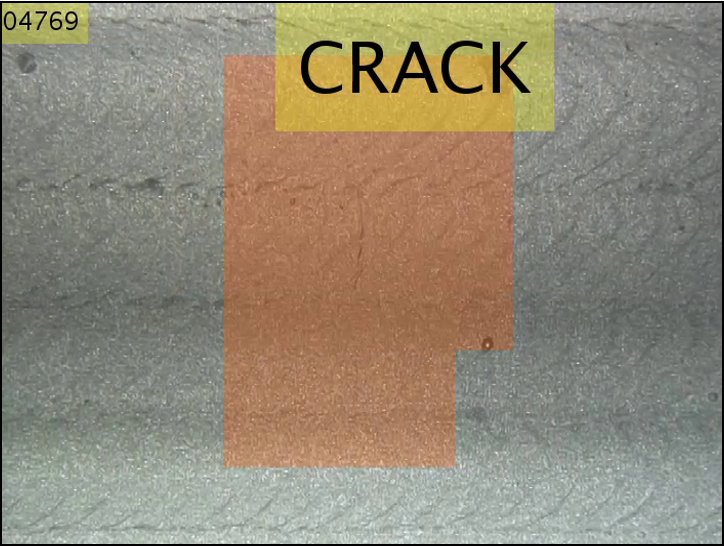
\includegraphics[width=0.43\textwidth,height=0.20\textheight]{Images/TPCrack3.png} &
                    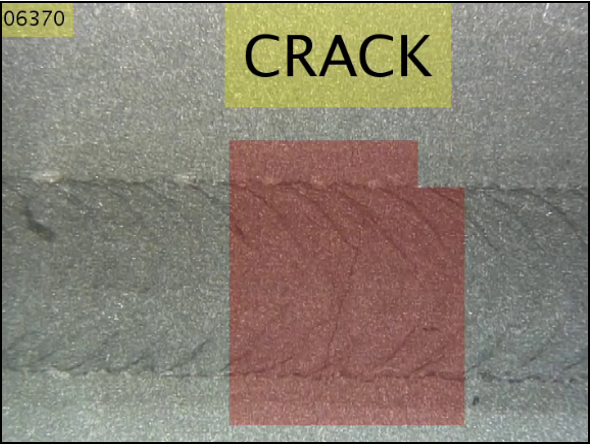
\includegraphics[width=0.43\textwidth,height=0.20\textheight]{Images/TPCrack4.png} \\
                    \multicolumn{2}{c}{(a) True positive cracks detections} \\
                    
                    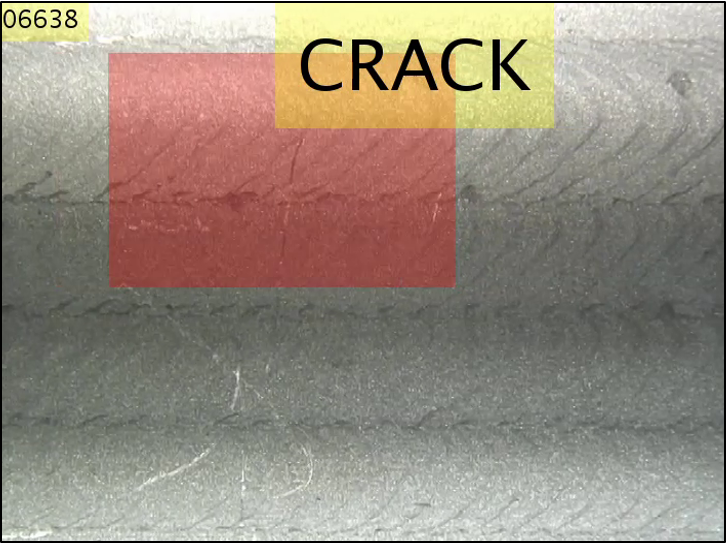
\includegraphics[width=0.43\textwidth,height=0.20\textheight]{Images/FPCrack3.png} &
                    
\includegraphics[width=0.43\textwidth,height=0.20\textheight]{Images/NoVisualHolder.png} \\
                    \multicolumn{2}{c}{(b) False positive cracks detections} \\
                    
                    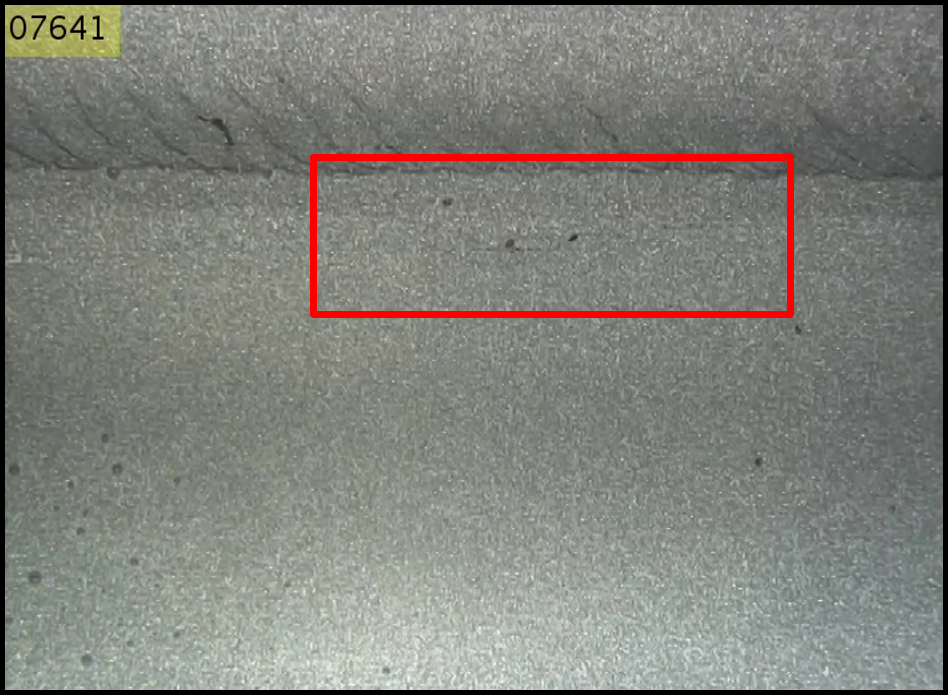
\includegraphics[width=0.43\textwidth,height=0.20\textheight]{Images/FNCrack3.png} & 
                    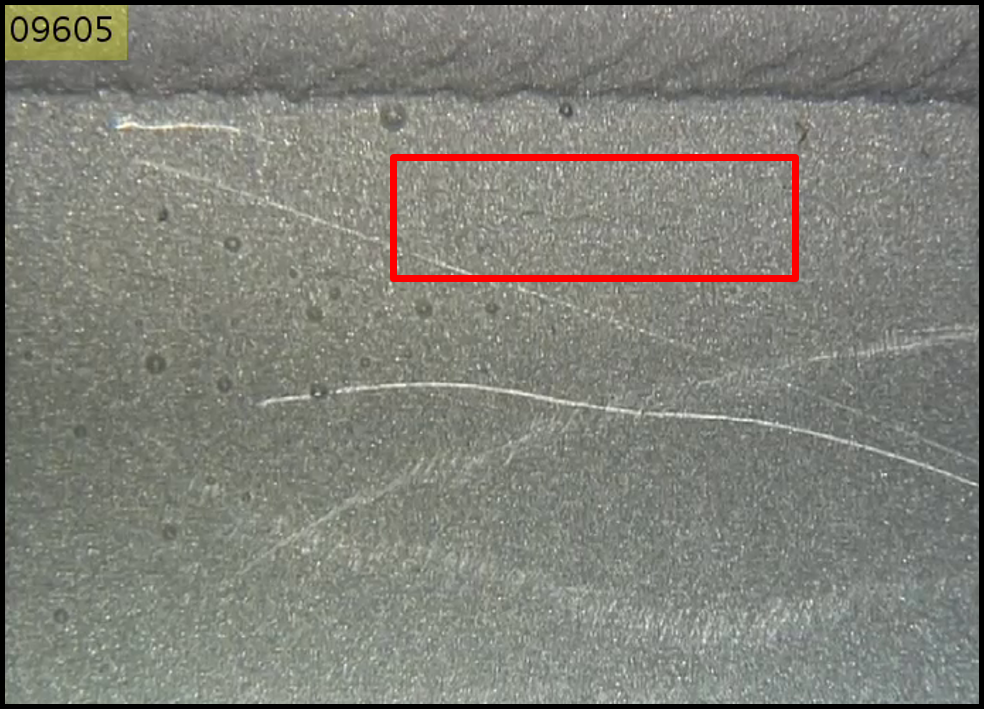
\includegraphics[width=0.43\textwidth,height=0.20\textheight]{Images/FNCrack4.png} \\
                    \multicolumn{2}{c}{(c) False negative cracks detections}
                % }
            \end{tabular}
            }
        % \end{centering}
        
        
        \caption{Classification examples of the proposed method. The images in the top each contained a single crack that was correctly identified. The images in the middle row contain no cracks but were falsely identified as crack images. The bottom row shows examples of difficult cracks that were missed.}
        \label{fig:FigExample}
        
    \end{figure*}
    
    %% ------------------------------------------------


\section{Overview}
    % We propose a method to reduce the number of false positives that does not sacrifice, but improves true detection rates on crack containing frames by leveraging spatial and temporal information of the inspection video.
    We refer to fix sized subregions of a video frame $f$ as an image patch $\patch$. For determining whether image patches potentailly contain a crack, a CNN is fine tuned with positive and negative patches taken from a manually labeled dataset \ref{detection}.  During testing, image patches classified as potentially containing cracks are represented as a 3$-$dimensional point cloud and grouped across all frames of the inspection video into special-temporal planes using RANSAC plane fitting \ref{planes}. These planes are then classified as crack containing planes or not through a dual-threshold method with statistically inferred thresholds, which in turn determines the predicted frames and regions in these frames containing cracks.  


    \subsection{Patch-Level Crack Detection} \label{detection}
            Given the set of frames $\vect{F}$ for a video, each frame $f \in \vect{F}$ is divided into 224x224 pixel patches where adjacent patches contain about 75\% overlap in area. This amount of overlap and block size allows for a finer classification grid across the frame image to be utilized in the spatial-temporal grouping described in \ref{planes}. The ImageNet mean RGB value is subtracted from each patch \comment{as in [X]} and then it is run through the fine-tuned CNN described in \ref{training} and classified as $y \in \{0,1\}$, where $y=1$ is a patch that possibly contains a crack.



    \subsection{Spatial-Temporal patch grouping} \label{planes}
            Let $\crackPatchSet$ be the set of patches classified as possibly containing a crack in all frames of the video as described in \ref{detection}. We define a set of potential crack points $\crackPoint \in \crackPointSet$ and perform RANSAC plane fitting and classify the planes to determine cracks at the frame level.

            \paragraph{Plan Fitting}
                Each $\patchi \in \crackPatchSet$ is represented as a 3D point $\crackPointi = (x, y, t)$ where $t$ is the frame number which the patch taken from and $(x,y)$ is the center of the patch. The set $\crackPointSet$ forms a 3D point cloud from where plans are iteratively fit using RANSAC \comment{[X]}. For each plane found, the inlier points of the found plane are removed, and RANSAC plane fitting is run again. This is done until no more planes are found.  For the settings for RANSAC plane fitting, a reference vector of [0, 0, 1] is used. It points approximately parallel to normal vectors of the desired planes with max angle offset between the two vectors of 15 degrees. Each inlier point of the plane has a maximum distance from the surface of the plane of about 500.
            
            \paragraph{Plan Classification} 
                Each plane $\planTerm$ found in during grouping is associated with a set of potential crack points, or $\planTerm = \{\crackPointi\}$ where $\crackPointi \in \crackPointSet$. We classify the planes to determine cracks at the frame level by applying a double threshold on the following features for a given $\planTermi$. Let $\vect{t^{*}}=\{t_i\}$ be the set of distinct time values in the set of crack points $\planTermi$, we can then define:
                \begin{enumerate}
                    \item  $\threshOneName(\planTermi) = \arg\max_{(j,k)}[|\crackPoint_j.t - \crackPoint_k.t|]$ 
                    \item  $\threshTwoName(\planTermi) = \frac{\vect{t^{*}}}{(span(l_i))}$
                \end{enumerate}
                where $\crackPoint_j$ and $\crackPoint_k$ are crack points in $\planTermi$. Frames within the interval of a plan $\planTermi$ are said to contain a crack if:
                
                \begin{gather}
                    \label{DualThresh}
                    \threshOneName(\planTermi) > \lambda_1 $ \text{ } \text{ and } $ \threshTwoName(\planTermi) > \lambda_2
                \end{gather}
                
                 We define the threshold values of $\lambda_1$ and $\lambda_2$ both as the mean minus two standard deviations of patches containing cracks in the training set for $\threshOneName$ and $\threshTwoName$ respectively. 
        
    


   
    
    
    
             



    \subsection{CNN training}
    \label{training}
        We utilize the effectivness of existing CNN classifers, adapted to crack the detection probelm domain, for determining potential cracks on image patches from the video frames. Specifically, a GoogLeNet CNN \comment{\cite{googlenet2014going}} is finetuned by retraining the final inner product layer of the CNN to determine if a image patch has a crack it or not. Approximately 1.5 million 224x224 image patches are extracted from 16 videos for each training set. Crack patches are selected from manually pixel labeled ground truthed crack frames with a crack pixel in the center of the patch. Additional crack patch samples are added by rotating the initial crops by  90 degrees. 
        Classification accuracy and performance during training can be improved by subsampling the non-crack patches based on a morphological response $T$ of the image patches. This is done by first applying to every non-crach patch a morphological operation similar to the approach proposed by Jahanshahi et. al \cite{jahanshahi2013}. $T$ for an image patch $p$ is defined as:
        
        \begin{equation}
                T = \max{[(p \circ \vect{s}) \bullet \vect{s}, p}] - p 
        \end{equation}
        
        where '$\circ$' is the morphological opening operation, '$\bullet$' is the morphological closing and $\vect{s} = S_{[0^o,45^o,90^o,135^o]}$ is the structuring element that defines which neighboring pixels are included in the operation. Weighted sampling, determined by the maximum response $T$ of each of the non-crack patches, is used to select a subsample from the non-crack patches for training. An equal number of positive and negative samples is used during training. The CNN produces a score for each possible classification class and the patch assigned a label from the highest class score as $y \in \{0,1\}$, where $y=1$ is a patch that possibly contains a crack.  
        
         
        \paragraph{Implementation Details}
             The CNN weights are initialized from the GoogLeNet that is available at the Caffe model zoo. The final inner product layer is the layer that is initialized from scratch. We use caffe \cite{jia2014} to finetune train the GoogLeNet by first subtracting mean RGB color of ImageNet from each of the training patches.  The blob learning rate coefficients of the final inner product layer are 10 times higher than the learning rate coefficients from the layers initialized from GoogLeNet.  The base learning rate. is set to  $0.001$,   gamma to $0.1$, momentum $0.9$, and weight decay $0.0005$.  We use a training batch size of 128 for each iteration for a total of 25,000 iterations.  A softmax classifier is attached to the final layer for classification.
    
    
    
         

